% Layout adapted from ../samplereport.tex. Compile twice with pdfLaTeX.
% VS Code/WSL: this folder auto-saves and builds with latexmk; preview uses build/.
\documentclass[11pt,a4paper]{article}
\usepackage[T1]{fontenc}
\usepackage{lmodern}
\usepackage{microtype}
\usepackage[top=3cm,bottom=3cm,left=2cm,right=2cm]{geometry}
\usepackage{amsmath,amssymb}
\usepackage{array,booktabs,tabularx}
\usepackage{graphicx}
\usepackage{fancyhdr}
\usepackage[table]{xcolor}
\usepackage{tikz}
\usepackage[hidelinks]{hyperref}

\newcommand{\UniversityLineOne}{VIETNAM NATIONAL UNIVERSITY HO CHI MINH CITY}
\newcommand{\UniversityLineTwo}{HO CHI MINH CITY UNIVERSITY OF TECHNOLOGY}
\newcommand{\FacultyName}{FACULTY OF COMPUTER SCIENCE AND ENGINEERING}
\newcommand{\ReportCourse}{Specialized Project (CO4029)}
\newcommand{\ReportTitle}{Improving 3D Gaussian Splatting for efficient and geometrically consistent 3D reconstruction, followed by conversion into editable polygon meshes}
\newcommand{\ReportSubtitle}{Gaussian reduction, surface constraints and mesh extraction}
\newcommand{\LecturerName}{Nguyen Tuan Khoi}
\newcommand{\StudentName}{Nguyen Vu Long}
\newcommand{\LogoFile}{figures/hcmut-logo.png}

\definecolor{ReportBlue}{HTML}{123D70}
\definecolor{ReportLight}{HTML}{EDF3F8}
\definecolor{ReportGray}{HTML}{526170}
\hypersetup{pdftitle={3D Gaussian Splatting Research Progress Report},
  pdfauthor={Nguyen Vu Long},pdfsubject={Specialized Project (CO4029)}}
\renewcommand{\contentsname}{TABLE OF CONTENTS}
\setcounter{tocdepth}{1}
\setlength{\headheight}{40pt}
\setlength{\parindent}{0pt}
\setlength{\parskip}{5pt}
\setlength{\emergencystretch}{1em}
\renewcommand{\arraystretch}{1.13}
\newcolumntype{Y}{>{\raggedright\arraybackslash}X}
\raggedbottom

\pagestyle{fancy}
\fancyhf{}
\fancyhead[L]{\begin{tabular}{@{}c@{\hspace{7pt}}l@{}}
  \raisebox{-0.40\height}{\includegraphics[width=8mm]{\LogoFile}} &
  \begin{tabular}{@{}l@{}}\footnotesize\bfseries\ttfamily\UniversityLineTwo\\
  \footnotesize\bfseries\ttfamily\FacultyName\end{tabular}
\end{tabular}}
\fancyfoot[L]{\scriptsize\ttfamily CO4029 / HK261}
\fancyfoot[R]{\scriptsize\ttfamily Page \thepage/\pageref*{report-end}}
\renewcommand{\headrulewidth}{0.3pt}
\renewcommand{\footrulewidth}{0.3pt}

\begin{document}
\hypersetup{pageanchor=false}
\begin{titlepage}
\centering
{\bfseries\UniversityLineOne\\[1mm]
\UniversityLineTwo\\[1mm]
\FacultyName\par}
\vspace{1cm}
\includegraphics[width=3cm]{\LogoFile}\par
\vspace{1cm}

\begin{minipage}{0.88\textwidth}
\raggedright
{\Large\bfseries\ReportCourse\par}
\vspace{0.55cm}
\hrule
\vspace{0.45cm}
{\small\bfseries\color{ReportGray} RESEARCH PROGRESS REPORT\par}
\vspace{0.22cm}
{\Large\bfseries\ReportTitle\par}
\vspace{0.16cm}
{\large\ReportSubtitle\par}
\vspace{0.45cm}
\hrule
\vspace{0.55cm}
\begin{tabular}{@{}ll@{}}
\textbf{Lecturer} & \LecturerName \\
\textbf{Student} & \StudentName{} (2352696) \\
\textbf{Email} & \href{mailto:long.nguyenty@hcmut.edu.vn}{long.nguyenty@hcmut.edu.vn} \\
\end{tabular}
\end{minipage}

\vspace{2cm}
{\small\bfseries Ho Chi Minh City\par}
\end{titlepage}
\hypersetup{pageanchor=true}

\begingroup
\setlength{\parskip}{0pt}
\tableofcontents
\endgroup

\clearpage
\section*{Executive summary}
This project extends gsplat to train more compact 3D Gaussian Splatting
(3DGS) models and to reconstruct personal recordings on a GTX 1660 SUPER
with 6 GB of VRAM. The work covers budgeted densification, RealSense RGB-D
pose recovery and depth supervision, a reconstruction viewer, an RGB-only
video pipeline, and conversion of optimized Gaussians into polygon meshes.
This revision consolidates saved experimental evidence; no experiments were
rerun for the report update. Technical repository deliverables are available,
while supervisor review and final mesh validation remain outstanding.

\medskip
{\small
\begin{tabularx}{\linewidth}{@{}p{0.25\linewidth}Y@{}}
\toprule
\textbf{Workstream} & \textbf{Progress and evidence} \\
\midrule
Gaussian allocation & A04 reduced mean Gaussian count by 24.25--35.27\%
across four indoor scenes and three paired seeds. Mean PSNR rose on all four
scenes, with the most consistent gains on Room and Counter. \\
A05 absolute gradients & Across Room, Counter and Kitchen at seeds 42/43,
PSNR improved and counts fell versus A04 in all six comparisons. Five of six
passed the practical gate; count reductions were 24.33--32.59\%. \\
Surface and meshes & A matched Room reduction $\times$ curvature-prior study
produced four raw Gaussian-derived PLY/OBJ meshes. Smoothness proxies improved,
but topology was mixed. Retain A05-Abs without the prior. \\
RealSense reconstruction & The 15 FPS RGB-D pipeline gained 1.41 dB PSNR
over the 2 FPS baseline on the same 79 held-out targets. Frame selection,
matching and pose optimization changed together. \\
Room geometry & An alternate RGB distortion mapping agreed with sampled SDK
coordinates within 0.029 pixels. Physical calibration and trajectory accuracy
still require independent validation. \\
Ordinary video & A controlled fixture reached GPU training after a diagnostic
gate change. The user video failed the registration gate at both sampled rates. \\
School milestones & Technical catch-up artifacts exist. Supervisor
presentation and feedback, mesh cleanup and editing validation remain pending. \\
\bottomrule
\end{tabularx}}

\subsection*{How results are evaluated}
PSNR measures pixel error on a logarithmic scale, SSIM compares image
structure, and LPIPS measures perceptual distance in learned features.
Higher PSNR and SSIM and lower LPIPS are preferred. Gaussian count describes
representation size, peak tensor allocation describes one aspect of GPU
memory use, and registered-view counts describe pose coverage. Physical
geometry requires separate calibration and trajectory checks.

\clearpage
\section{Datasets and exploratory data analysis}
\label{sec:datasets}
The experiments use public multi-view photographs, a synthetic scene, three
RealSense captures and one user video. Several experiments reuse the same
source observations at different resolutions or frame rates. The audit
counts these as variants of their source, and distinguishes selected frames,
registered frames and the images actually used in training or evaluation.

\subsection{Public scenes and CCD-GS fixtures}
The A04 study uses the four indoor scenes from Mip-NeRF 360
\cite{mipnerf360}, with the released half-resolution images and SfM
initialization. The parser sorts image names and holds out every eighth view,
starting at index zero. Each A04--B00 comparison uses the same split. The
CCD-GS pilot uses the same Room views at one-eighth resolution and a synthetic
scene of three textured or colored spheres above a checkerboard, rendered
with known cameras. CCD-GS measures split utility on development images and
reserves a separate test split. The benchmark Room and the later RealSense
room are different scenes.

\begin{table}[!ht]
\centering\small
\begin{tabularx}{\linewidth}{@{}Ylrrrrr@{}}
\toprule
\textbf{Scene} & \textbf{Image size} & \textbf{Total} & \textbf{Train} & \textbf{Dev.} & \textbf{Held out} & \textbf{Initial points} \\
\midrule
Room & $1557\times1038$ & 311 & 272 & -- & 39 & 112,627 \\
Counter & $1558\times1038$ & 240 & 210 & -- & 30 & 155,767 \\
Kitchen & $1558\times1039$ & 279 & 244 & -- & 35 & 241,367 \\
Bonsai & $1559\times1039$ & 292 & 255 & -- & 37 & 206,613 \\
Room, CCD-GS & $389\times259$ & 311 & 233 & 39 & 39 & 112,627 \\
Analytic spheres & $128\times128$ & 48 & 36 & 6 & 6 & 1,280 \\
\bottomrule
\end{tabularx}
\caption{Public and synthetic image splits.}
\label{tab:benchmark-data}
\end{table}

\subsection{RGB audit of public and synthetic images}
For each input set, the audit reads up to 48 evenly spaced file indices
after sorting by name. It converts images to 8-bit grayscale and downsamples
the long side to at most 384 pixels using box filtering. Luma is the mean
pixel intensity per frame on a 0--255 scale. The median variance of a
four-neighbor Laplacian indicates image detail and responds to texture,
noise and resampling as well as blur.

\begin{table}[!ht]
\centering\small
\begin{tabularx}{\linewidth}{@{}Yrrr@{}}
\toprule
\textbf{Scene} & \textbf{Luma p10--p90} & \textbf{Median luma} & \textbf{Median Laplacian variance} \\
\midrule
Room & 61--106 & 76 & 632 \\
Counter & 67--99 & 80 & 988 \\
Kitchen & 112--135 & 128 & 1,595 \\
Bonsai & 50--104 & 64 & 1,039 \\
Room, CCD-GS & 61--105 & 76 & 696 \\
Analytic spheres & 63--67 & 65 & 3,622 \\
\bottomrule
\end{tabularx}
\caption{Sampled RGB statistics for public and synthetic images.}
\label{tab:benchmark-rgb}
\end{table}

Kitchen is the brightest benchmark scene in the sample, while Bonsai has
the widest luma spread. The analytic fixture has a narrow luma spread and
high-frequency checkerboard edges at its native 128-pixel scale. It offers
controlled pose evidence on simpler imagery than the captured scenes.

\clearpage
\subsection{RealSense captures and data splits}
Each capture pairs RGB images with depth from a separate sensor and uses
calibration to project valid depth into the RGB camera. The first indoor
indoor capture lasted 346.9 s. Its two sampling passes selected 694 and
5,204 frames. The courtyard capture stored 6,996 RGB frames over
233.4 s, including passes with and without people. The exhibit-room
capture stored 4,764 frames over 159.0 s in an indoor exhibit room with
bright openings and reflective surfaces.

\begin{table}[!ht]
\centering\small
\begin{tabularx}{\linewidth}{@{}Yrrrrr@{}}
\toprule
\textbf{Dataset variant} & \textbf{Selected} & \textbf{Posed} & \textbf{Train} & \textbf{Held out} & \textbf{Withheld} \\
\midrule
Indoor capture, pilot at 2 FPS & 694 & 113 & 98 & 15 & 0 \\
Indoor capture, native-resolution at 2 FPS & 694 & 151 & 132 & 19 & 0 \\
Indoor capture, broad at 2 FPS & 694 & 626 & 547 & 79 & 0 \\
Indoor capture, broad at 15 FPS & 5,204 & 5,201 & 4,740 & 79 & 382 \\
\addlinespace
Courtyard at 3 FPS & 701 & 701 & 613 & 88 & 0 \\
Courtyard at 30 FPS, original and corrected poses & 6,996 & 6,996 & 5,970 & 88 & 938 \\
Courtyard, people-preference variant & 6,996 & 6,996 & 5,544 & 88 & 1,364 \\
Courtyard stairs, local pose trial & 28 & 28 & 23 & 3 & 2 \\
\addlinespace
Exhibit room at 3 FPS, baseline and SDK remap & 477 & 477 & 417 & 60 & 0 \\
\bottomrule
\end{tabularx}
\caption{RealSense coverage and image roles.}
\label{tab:rgbd-splits}
\end{table}

In Table~\ref{tab:rgbd-splits}, \emph{posed} counts frames in the dataset's
recovered camera model. \emph{Withheld} counts posed frames outside the training
and held-out sets, including temporal buffer frames. For the 15 FPS run, the
split lists 4,743 training names, but three failed registration. The 30,000
recorded training updates visited all 4,740 available training views.
The 2 FPS broad run averaged 54.8 updates per training view, compared with
6.3 at 15 FPS. The additional frames increase observation density and
spread the same training budget across more views.

\medskip
\textbf{Matched targets.} The indoor capture broad runs share 79 original RGB
targets. The courtyard runs share 88 targets, and the full-rate variants
omit training observations within 0.2 s of them. The people-preference
trial excludes another 426 training frames. The stairs subset spans
9.28 s and reserves two buffer frames using a 0.3 s rule. The exhibit room
variants retain the same 60 held-out source identities under the two RGB
mappings. These splits measure image quality on frames withheld from
Gaussian training, using poses estimated jointly with the other views.

\medskip
\textbf{Pose coverage depends on the pipeline.} RGB-only mapping registered
113 of 694 indoor capture views before retrieval and depth-backed bridging, 431 of
701 courtyard views and 301 of 477 exhibit-room views in their largest
components. The final RGB-D models recover more camera locations, with
the exhibit and courtyard datasets retaining all selected views. These
counts describe camera coverage along the captured path.

\clearpage
\subsection{RealSense timing, depth and RGB variation}
Frame gaps below are computed from consecutive RGB timestamps in the
capture manifests. The depth fraction is the share of source depth pixels
that survive the recorded depth filter. The pairing gap is the absolute
difference between the selected RGB and depth timestamps.

\begin{table}[!ht]
\centering\small
\begin{tabularx}{\linewidth}{@{}Yrrr@{}}
\toprule
\textbf{Capture or subset} & \textbf{RGB gap p50/p95 (ms)} & \textbf{Valid depth p10/p50/p90 (\%)} & \textbf{Pair p95 (ms)} \\
\midrule
Indoor capture, 2 FPS & 501 / 701 & -- & -- \\
Indoor capture, 15 FPS & 67 / 101 & -- & -- \\
Courtyard, 3 FPS & 334 / 634 & 26.7 / 42.9 / 71.4 & 8.65 \\
Courtyard, 30 FPS & 33 / 35 & 27.0 / 43.5 / 71.9 & 8.64 \\
Courtyard stairs & 333 / 635 & 32.5 / 48.3 / 55.8 & 8.19 \\
Exhibit room, 3 FPS & 334 / 634 & 40.7 / 70.3 / 87.3 & 7.91 \\
\bottomrule
\end{tabularx}
\caption{RealSense timing and source-depth availability.}
\label{tab:rgbd-metadata}
\end{table}

The indoor capture manifests omit directly comparable valid-pixel fractions and
pairing gaps. In 48 sampled depth-cache files at each rate, the median of
the per-frame median depths was about 0.82 m at both rates. Each sampled cache file
contains 12,000 retained depth points, so it provides a depth distribution
after sampling. The courtyard median valid depth remains near 43\% at both
rates, and about 3\% of full-rate frames fall below 20\% valid depth. The
exhibit room has more usable depth overall, but its p10 is only 40.7\%.
The SDK remap uses the same source-depth manifest.

\begin{table}[!ht]
\centering\small
\begin{tabularx}{\linewidth}{@{}Ylrr@{}}
\toprule
\textbf{Prepared RGB input} & \textbf{Image size} & \textbf{Luma p10--p90} & \textbf{Near-white pixels (\%)} \\
\midrule
Indoor capture, pilot at 2 FPS & $848\times475$ & 79--120 & 1.87 \\
Indoor capture, native-resolution & varies$^{\ast}$ & 74--116 & 1.99 \\
Indoor capture, broad at 2 FPS & $848\times477$ & 39--105 & 2.29 \\
Indoor capture, broad at 15 FPS & $848\times477$ & 42--101 & 2.05 \\
Courtyard, 3 FPS & $834\times463$ & 89--127 & 1.17 \\
Courtyard, 30 FPS & $834\times463$ & 85--124 & 1.05 \\
Courtyard stairs & $834\times463$ & 95--120 & 0.81 \\
Exhibit room baseline & $834\times463$ & 96--130 & 4.47 \\
Exhibit room SDK remap & $834\times463$ & 96--131 & 4.49 \\
\bottomrule
\end{tabularx}
\caption{Sampled RGB statistics for prepared RealSense inputs.}
\label{tab:rgbd-rgb}
\end{table}

Near-white is the median per-frame share of resized grayscale pixels at
intensity 250 or higher. All 28 stairs views were read. The other rows use
48 images each. $^{\ast}$The native export has 115 images at $1278\times716$
and 36 at $1277\times717$. The broad indoor capture datasets include darker views
than the smaller RGB reconstructions. The exhibit room has the most
near-white pixels in this audit, consistent with bright openings and glare.

\clearpage
\subsection{RGB-only video and temporal registration}
The workflow fixture is a 48-frame clip made from low-resolution Mip-NeRF
360 Room images. It checks extraction, mapping, training and viewer
integration. The user video, a portrait MP4, is a separate
portrait recording of about 11.2 minutes. Both real-video runs use the
same RGB-only mapping approach, with a single estimated camera model.

\begin{table}[!ht]
\centering\small
\begin{tabularx}{\linewidth}{@{}Ylrrrr@{}}
\toprule
\textbf{Input} & \textbf{Image size} & \textbf{FPS} & \textbf{Extracted} & \textbf{Largest model} & \textbf{Share} \\
\midrule
Workflow fixture & $640\times426$ & 2 & 48 & 28 & 58.3\% \\
User video, sparse sampling & $540\times960$ & 2 & 1,339 & 118 & 8.8\% \\
User video, dense sampling & $540\times960$ & 30 & 20,090 & 4,072 & 20.3\% \\
\bottomrule
\end{tabularx}
\caption{RGB-only video extraction and registration.}
\label{tab:video-data}
\end{table}

The 48-image samples give luma p10--p90 of 58--97 for the fixture, 81--125
for the user video at 2 FPS and 82--119 at 30 FPS. Median Laplacian variance
was 271, 464 and 600, respectively. These differences describe the sampled
images. They combine content, texture and sampling effects.

\begin{figure}[!ht]
\centering
\begin{tikzpicture}[x=1.08cm,y=0.038cm,font=\small]
  \foreach \y in {0,25,50,75,100} {
    \draw[ReportGray!25] (0.5,\y) -- (10.5,\y);
    \node[anchor=east,text=ReportGray] at (0.46,\y) {\y};
  }
  \draw[ReportGray] (0.5,0) -- (10.5,0);
  \foreach \x/\sparse/\dense in {
    1/0/0,2/0/0,3/0/0,4/0/0,5/0/0,6/0/0,7/14.18/14.24,
    8/57.46/62.12,9/16.42/47.29,10/0/79.04} {
    \fill[ReportGray!57] (\x-0.35,0) rectangle (\x-0.03,\sparse);
    \fill[ReportBlue] (\x+0.03,0) rectangle (\x+0.35,\dense);
    \node[below] at (\x,0) {\x};
  }
  \node[rotate=90] at (-0.38,50) {Registered frames (\%)};
  \node[below] at (5.5,-12) {Consecutive frame deciles, start to end};
  \fill[ReportGray!57] (6.8,109) rectangle (7.08,116);
  \node[anchor=west] at (7.12,112.5) {2 FPS};
  \fill[ReportBlue] (8.65,109) rectangle (8.93,116);
  \node[anchor=west] at (8.97,112.5) {30 FPS};
\end{tikzpicture}
\caption{User-video coverage in the largest COLMAP model at each rate.}
\label{fig:video-coverage}
\end{figure}

Each bar divides the registered frames by all extracted frames in that
segment. Both largest models begin around 7 min 39 s into the clip, so
their registrations are concentrated in the final third. The denser run
reaches more of the ending, yet both runs fail the 80\% gate. The fixture
also fails the default threshold, with frames 21--48 in its largest model.
It reaches a short GPU smoke run only under the diagnostic 50\% threshold.

\clearpage
\section{Budgeted Gaussian densification}
\label{sec:allocation}
3DGS represents a scene as soft, translucent ellipsoids with learned size,
orientation, opacity and view-dependent color~\cite{kerbl,gsplat}.
\emph{Densification} gives the scene more detail by cloning or splitting
existing Gaussians during training. Since both operations increase the
model size, the project separates three decisions: how many Gaussians to
add, which parents to select, and how to initialize their children.

\subsection{How many Gaussians to add}
Inspired by Taming 3DGS~\cite{taming}, \texttt{BudgetStrategy} sets a live
count target at each eligible refinement event. Let $N_0$ be the initial
count, $N_{\max}$ the cap, and $u$ the fraction of eligible refinement
events through the current one. The target and number of growth slots are
\begin{equation}
  \begin{aligned}
    N_{\mathrm{target}}(u)&=\bigl\lfloor N_0+(N_{\max}-N_0)(2u-u^2)\bigr\rfloor,\\
    K&=\min\bigl(\max(0,N_{\mathrm{target}}-N_{\mathrm{live}}),\ N_{\mathrm{eligible}}\bigr).
  \end{aligned}
  \label{eq:budget}
\end{equation}
The schedule permits 75\% of the total growth halfway through the events,
giving early children more time to train. Each clone adds one Gaussian.
Each split replaces one parent with two children, also adding one. Pruning
then removes Gaussians, so the final count can fall below the cap. During
parameter replacement, old and new tensors can briefly coexist in memory.

\textbf{Example.} Starting with 100,000 Gaussians and a 700,000 cap gives a
550,000 target at $u=0.5$. With 540,000 live Gaussians and 6,000 eligible
parents, Eq.~\eqref{eq:budget} allocates 6,000 slots. The count reaches
546,000 before pruning.

\subsection{Which parents receive growth slots}
Eligibility comes first. The average magnitude of the screen-space position
gradient must exceed a threshold, or a projected radius must exceed its
threshold while that size check is active. Candidates below the opacity
pruning threshold are excluded. The strategy ranks the remaining candidates
and selects the top $K$.

\textbf{A01 uses gradient.} The screen-space gradient measures how sensitive
the training loss is to moving the projected Gaussian. Larger values suggest
that the image fit is sensitive to the primitive's position.

\textbf{A02 adds attributed RGB error.} Every ten training steps in the
refinement window, the renderer reuses the current projections to find the
four strongest contributors to each pixel. Their blend weights are
$w_i(p)=T_i(p)\alpha_i(p)$, where $T_i$ is the fraction of light that passes
through nearer splats and $\alpha_i$ is this splat's opacity at the pixel. Each receives
the pixel's mean absolute RGB error multiplied by $w_i(p)$. A splat with
weight 0.6 at a pixel with error 0.2 receives 0.12 before aggregation.

\textbf{A03 adds edge detail.} The same attribution weights distribute the
absolute grayscale Laplacian of the target image, a measure of local
intensity change that highlights fine boundaries and texture.

Error and edge sums are averaged over contributing observations. Each
signal is scaled by its positive median among eligible candidates and
clipped at 20. The A03 and A04 ranking combines the normalized gradient
with the normalized error and one quarter of the normalized edge term.
The latter two receive a support multiplier $\sqrt{\min(m/3,1)}$ for $m$
contributing observations. Attribution resets at each growth event so the
children begin with fresh evidence. The score estimates where more detail
may help from the current renders.

\clearpage
\subsection{Long-Axis Split}
A01 through A03 retain the default clone-or-split rule. It generally clones
small selected parents and replaces larger ones with randomly offset
children. A04 keeps the A03 score and adapts the Long-Axis Split of Deng
et al.~\cite{improved} for all selected parents, including small ones.

\begin{enumerate}
  \setlength{\itemsep}{3pt}
  \item \textbf{Place two children symmetrically.} For parent center $\mu$,
  longest scale $s_k$ and corresponding unit axis $v_k$, place the centers
  at $\mu\pm\delta v_k$, with $\delta=3d\,s_k$ and $d=0.45$.
  \item \textbf{Shrink each child.} Each child uses a scale multiplier
  of $1-d=0.55$ along the longest axis and $\sqrt{1-d^2}\approx 0.89$ on
  the two transverse axes. Both inherit the parent's rotation.
  \item \textbf{Carry over appearance.} Copy the parent's spherical-harmonic
  color coefficients and initialize each child's opacity at 60\% of the
  parent's activated opacity.
\end{enumerate}

\begin{figure}[!ht]
\centering
\begin{tikzpicture}[font=\small]
  \node[font=\small\bfseries] at (0,0.96) {Parent};
  \node[font=\small\bfseries] at (6.3,0.96) {Children};
  \draw[draw=ReportBlue,fill=ReportLight,thick] (0,0)
    ellipse[x radius=1.45cm,y radius=0.58cm];
  \draw[draw=ReportBlue,fill=ReportLight,thick] (5.03,0)
    ellipse[x radius=0.80cm,y radius=0.52cm];
  \draw[draw=ReportBlue,fill=ReportLight,thick] (7.57,0)
    ellipse[x radius=0.80cm,y radius=0.52cm];
  \draw[densely dashed,ReportGray] (-1.65,0) -- (1.65,0);
  \draw[densely dashed,ReportGray] (4.12,0) -- (8.48,0);
  \draw[dotted,ReportGray] (6.3,-0.52) -- (6.3,0.52);
  \draw[->,thick,ReportBlue] (2.02,0) -- (3.74,0)
    node[midway,above] {Split};
  \fill[ReportBlue] (0,0) circle[radius=2pt];
  \fill[ReportBlue] (5.03,0) circle[radius=2pt];
  \fill[ReportBlue] (7.57,0) circle[radius=2pt];
  \node at (0,-0.83) {$\mu$};
  \node at (5.03,-0.83) {$\mu-\delta v_k$};
  \node at (6.3,-0.83) {$\mu$};
  \node at (7.57,-0.83) {$\mu+\delta v_k$};
\end{tikzpicture}
\caption{Long-Axis Split shown in the parent's principal plane.}
\label{fig:long-axis}
\end{figure}

The parent center remains the midpoint, and the shorter, less opaque
children aim to limit the change in the rendered footprint
(Fig.~\ref{fig:long-axis}). A diagnostic split the same large parents from
a frozen A03 checkpoint and compared the new renders with the pre-split
renders on four held-out views. Long-Axis Split produced 29.31\% less RGB
mean squared change than the average of three random placements. The
diagnostic ended before any recovery updates.

\subsection{How the cap affected the Room run}
At A04's final refinement event, 593,651 Gaussians were live. The 700,000
cap left 106,349 growth slots, but only 4,598 parents qualified. Splitting
those parents and pruning 260 Gaussians produced the final count of
597,989 in Table~\ref{tab:room-historical}.

\begin{table}[!ht]
\centering\small
\begin{tabularx}{\linewidth}{@{}Yrrrrr@{}}
\toprule
\textbf{Variant} & \textbf{Gaussians} & \textbf{PSNR (dB)} & \textbf{SSIM} & \textbf{LPIPS} & \textbf{Peak tensor GiB} \\
\midrule
B00 Original strategy    & 841,017 & 30.0335 & 0.90206 & 0.21165 & 1.280 \\
A01 Budget and gradient  & 699,173 & 29.7823 & 0.89855 & 0.21555 & 1.101 \\
A02 Add attributed error & 699,266 & 29.8630 & 0.90130 & 0.21299 & 1.104 \\
A03 Add edge detail      & 699,207 & 30.0166 & 0.90117 & 0.21405 & 1.116 \\
\rowcolor{ReportLight}
A04 Long-Axis Split      & 597,989 & 30.5058 & 0.90561 & 0.20486 & 1.062 \\
\bottomrule
\end{tabularx}
\caption{Historical Room densification results.}
\label{tab:room-historical}
\end{table}

\clearpage
\section{Densification results and limits}
The historical Room run used one seed and 7,000 updates at
$1{,}557\times1{,}038$, with 272 training and 39 held-out images.
A02 improved all three image metrics over A01.
A03 recovered further PSNR and used 16.86\% fewer Gaussians than B00,
with slightly worse SSIM and LPIPS. A04 improved all three metrics over
B00 with 28.90\% fewer Gaussians and 17.05\% lower peak tensor allocation
(Table~\ref{tab:room-historical}).

\subsection{Four-scene paired comparison}
The later campaign matched initialization and the full 7,000-view sampling
sequence within each scene and seed. Seeds 42, 43 and 44 were analyzed as
pairs. Historical runs were excluded from the averages.

\begin{figure}[!ht]
\centering
\begin{tikzpicture}[x=5.7cm,y=0.60cm,font=\small]
  \foreach \x in {-0.75,-0.50,-0.25,0,0.25,0.50,0.75} {
    \draw[ReportGray!20] (\x,0.5) -- (\x,4.5);
    \node[below,text=ReportGray] at (\x,0.5) {$\x$};
  }
  \draw[densely dashed,ReportGray] (0,0.5) -- (0,4.55);
  \node[anchor=west,text=ReportGray] at (0.89,4.68) {Count reduction};
  \foreach \name/\y/\low/\mean/\high/\reduction in {
    Room/4/0.3599/0.5688/0.7777/28.37,
    Counter/3/0.0807/0.1361/0.1916/24.25,
    Kitchen/2/-0.1458/0.1297/0.4052/35.27,
    Bonsai/1/-0.7378/0.0298/0.7975/32.31} {
    \node[anchor=east] at (-0.82,\y) {\name};
    \draw[ReportBlue,thick] (\low,\y) -- (\high,\y);
    \draw[ReportBlue,thick] (\low,\y-0.12) -- (\low,\y+0.12);
    \draw[ReportBlue,thick] (\high,\y-0.12) -- (\high,\y+0.12);
    \fill[ReportBlue] (\mean,\y) circle[radius=2.4pt];
    \node[anchor=west] at (0.89,\y) {\reduction\%};
  }
  \node[below] at (0,-0.23) {Mean PSNR change, A04 minus B00 (dB)};
\end{tikzpicture}
\caption{A04 versus B00, three paired seeds per scene. Dots show the paired
means and bars show 95\% Student's $t$ intervals ($2$ degrees of freedom).
The count column reports mean reduction.}
\label{fig:seed-results}
\end{figure}

Mean gains were +0.5688 dB on Room, +0.1361 on Counter, +0.1297 on
Kitchen and +0.0298 on Bonsai. Kitchen and Bonsai intervals include zero
(Fig.~\ref{fig:seed-results}). Mean SSIM increased and mean LPIPS decreased on
all four scenes. At the view level, A04 increased MSE on 20 of 35 Kitchen
views and 14 of 37 Bonsai views in the crop-study comparison. The evidence
covers four indoor scenes, and the three-seed intervals are imprecise.

\subsection{Ablation, budget and rejected mechanism}
\textbf{Split ablation.} On Room, mean PSNR was 30.1286 dB for random
splitting with small-parent cloning, 30.2922 for random splitting without
cloning, 30.4250 for long-axis splitting with cloning, and 30.6327 for
long-axis splitting without cloning. Both changes were associated with
gains. The operator comparison bundles placement, scale and opacity.

\textbf{Budget and tuning.} In one Room seed, caps of 400k, 700k and 1M gave
final counts of 399,842, 597,975 and 604,705 at 30.5461, 30.6007 and
30.6049 dB, respectively. A development grid selected $d=0.30$ and opacity
multiplier 0.40. Confirmation runs had mixed PSNR and worse LPIPS in all
three checks, so the frozen A04 setting remains the reference.

\textbf{CCD-GS pilot.} A bounded pose adjustment tested whether persistent
growth gradients predicted a useful split. Matched split/no-split
continuations and simpler gradient, multiview and pose-compute controls
tested that hypothesis. Zero of 36 checkpoint blocks met the prespecified
practical gate.

\clearpage
\section{A05 progression and candidate selection}
\label{sec:a05}
\subsection{Residual fallback: useful screen, unsupported ranking claim}
The A04 eligibility audit found unused scheduled growth slots late in
training. The first A05 variant therefore allowed up to 512 additional
opaque, below-gradient-threshold parents per event at steps 5000--5900,
using attributed RGB residuals supported by at least three distinct training
images. Ordinary A04 growth retained priority under the same 700k cap.

At the final archived seed-42 weights, a frozen-weight observation pass
selected 512 parents by residual or by gradient. Both branches and a
no-extra-split control used fresh Adam state and 500 matching continuation
updates. Residual selection lost to both controls on all three scenes:
PSNR differences versus no extra splits were $-0.01085$, $-0.01637$ and
$-0.03395$ dB for Room, Counter and Kitchen. It also trailed equal-count
gradient selection by $0.00638$, $0.01255$ and $0.02937$ dB. This intervention
tests converged weights, not the originally proposed late-training checkpoints.

The normal 7k-update seed-42 screen gained $+0.00626$, $+0.05222$ and
$+0.12737$ dB versus A04, respectively, with 7,499, 5,810 and 4,261 more
live Gaussians. Counter and Kitchen passed the practical gate; Room did not.
These common-cap gains do not establish that residual ranking is superior:
the equal-count intervention was negative and the end-to-end screen used
one seed. The residual method remains an opt-in experiment.

\subsection{Absolute-gradient alternative}
A05-Abs combines A04's budget, attributed-error/edge ranking and Long-Axis
Split with the existing absolute positional-gradient path. Absolute gradients
address cancellation before the eligibility decision, following the motivation
of AbsGS~\cite{absgs}. The policy sets \texttt{absgrad=True}, raises
\texttt{grow\_grad2d} to 0.0008 and disables residual fallback. Both the gradient
signal and threshold changed, so their separate effects are not isolated.

All runs use 7,000 updates, a 700k cap, original image splits and paired
archived A04 controls. Initialization and complete camera-sequence hashes
match. The frozen practical gate requires at least $+0.05$ dB PSNR, SSIM
loss at most 0.001 and LPIPS increase at most 0.001. All seed-42 scenes
passed, triggering the predeclared seed-43 confirmation.

\begin{table}[!ht]
\centering\small
\begin{tabularx}{\linewidth}{@{}Yrrrrrr@{}}
\toprule
\textbf{Scene / seed} & \textbf{PSNR} & \textbf{$\Delta$PSNR} & \textbf{$\Delta$SSIM} & \textbf{$\Delta$LPIPS} & \textbf{Gaussians} & \textbf{Pass} \\
\midrule
Room / 42 & 30.73701 & +0.13633 & +0.003950 & -0.010731 & 452,485 & Yes \\
Counter / 42 & 27.83983 & +0.09056 & -0.000634 & -0.001025 & 381,228 & Yes \\
Kitchen / 42 & 30.21228 & +0.22258 & -0.000247 & -0.000454 & 502,536 & Yes \\
Room / 43 & 30.81184 & +0.09168 & +0.003616 & -0.010074 & 442,656 & Yes \\
Counter / 43 & 27.77439 & +0.04191 & -0.000633 & -0.000017 & 384,975 & No \\
Kitchen / 43 & 30.05212 & +0.25887 & +0.000158 & -0.000131 & 508,135 & Yes \\
\bottomrule
\end{tabularx}
\caption{A05-Abs results. Deltas are candidate minus paired A04; PSNR is in dB.}
\label{tab:a05}
\end{table}

Counts fell 24.33--32.59\%; five pairs passed. Counter seed 43 missed the
PSNR threshold by 0.00809 dB; its SSIM fell about 0.00063 at both seeds.
Seed-42 peak tensor allocation fell from
1.080/1.090/1.229 to 0.971/0.945/1.077 GiB for Room/Counter/Kitchen;
training timers were similar. Audits verified finite checkpoints, PLY counts,
sources and 104 identical evaluation targets per seed. Exposed development
views and two seeds limit generalization. A05-Abs is the main reduced-model
candidate; A04 remains the paired reference.

\clearpage
\section{Surface constraints and optimized-Gaussian meshes}
\label{sec:surface}
\subsection{Completed Room factorial experiment}
The school objective includes geometrically consistent reconstruction and
editable polygon meshes. Earlier RealSense point-cloud meshes did not
complete conversion from optimized Gaussians. The new experiment crosses
baseline versus A05-Abs reduction with a surface-prior weight of zero versus
0.01, activated from update 3000. It uses Room seed 42 and 7,000 updates:
two verified archived no-prior controls and two new prior arms.

The optional prior penalizes horizontal and vertical second differences of
expected log depth. Images are sampled with stride four; detached RGB-edge
weights suppress penalties across image edges, and valid three-pixel
neighborhoods require finite positive depth and opacity above 0.7. This
encourages local smoothness without supervising physical surface locations.
It can still smooth incorrect or blended depth.

\begin{table}[!ht]
\centering\small
\begin{tabularx}{\linewidth}{@{}Yrrrr@{}}
\toprule
\textbf{Arm} & \textbf{PSNR} & \textbf{SSIM} & \textbf{LPIPS} & \textbf{Gaussians} \\
\midrule
Baseline & 29.99812 & 0.901684 & 0.209726 & 831,326 \\
Baseline + prior & 30.05953 & 0.902064 & 0.210307 & 827,764 \\
A05-Abs & 30.73701 & 0.909146 & 0.192058 & 452,485 \\
A05-Abs + prior & 30.73650 & 0.909322 & 0.191455 & 450,398 \\
\bottomrule
\end{tabularx}
\caption{Matched Room reduction $\times$ surface-prior study.}
\label{tab:surface-render}
\end{table}

All four arms match initialization and all 7,000 training-camera indices.
Each new arm's 39 evaluation targets match its control byte for byte;
initial metrics agree within 0.0001 and final tensors are finite. Both
prior comparisons pass the recorded rendering guardrails. On five fixed
held-out views using identical all-arm opacity support, mean edge-aware
log-depth curvature fell from 0.00541200 to 0.00514657 ($-4.90\%$) for the
baseline and from 0.00544199 to 0.00527539 ($-3.06\%$) for A05-Abs. This is
a smoothness proxy, not an independent geometric accuracy measurement.

\clearpage
\subsection{Chosen extraction route and raw asset quality}
Expected depth and RGB rendered from the optimized checkpoint at 64 training
cameras are fused into a bounded uniform TSDF, followed by surface extraction.
No sensor points or held-out depths are fused. All four arms share a cube
around the SfM 1st--99th percentile bounds enlarged 20\%, a target voxel size
of $0.01\times$ scene scale, resolution capped at 192 and truncation of four
actual voxels. Per-arm records preserve bounds, actual voxel size, source
hashes, topology and extraction timings.

\begin{table}[!ht]
\centering\small
\begin{tabularx}{\linewidth}{@{}Yrrrr@{}}
\toprule
\textbf{Raw mesh} & \textbf{Vertices} & \textbf{Triangles} & \textbf{Components} & \textbf{Boundary edges} \\
\midrule
Baseline & 69,337 & 119,613 & 1,241 & 18,165 \\
Baseline + prior & 65,638 & 114,598 & 1,131 & 15,804 \\
A05-Abs & 68,867 & 119,987 & 1,162 & 16,807 \\
A05-Abs + prior & 69,109 & 119,400 & 1,216 & 17,700 \\
\bottomrule
\end{tabularx}
\caption{Common-settings raw mesh extraction; counts do not establish accuracy.}
\label{tab:surface-mesh}
\end{table}

All four five-view comparison sheets were inspected. Major room structures
and furniture silhouettes are recognizable, but holes remain near edges,
thin furniture and plant details fragment, and tabletop details can merge.
The prior improves the curvature proxy while increasing A05-Abs component
and boundary-edge counts. A general continuity or accuracy improvement is
therefore unsupported. Retain A05-Abs with \texttt{surface\_lambda=0} as the
main candidate and preserve the prior as a studied alternative. Only two
weights were compared; exhaustive tuning is not claimed.

\subsection{Failures, corrections and reproducibility}
Four Windows workers duplicated decoded image caches and exhausted available
memory. Zero workers reduced memory use, but changed camera order after the
first epoch. The first full run failed pairing and remains a diagnostic under
\href{run:results/school_completion_20261109}{\texttt{results/school\_completion}}; its metrics are excluded from the
controlled effect. Explicit replay of the archived 7,000-camera sequence
restored checkable pairing in the accepted campaign.

The local Open3D 0.20 scalable TSDF returned no voxels even for a known flat
plane. Uniform TSDF recovered the plane and passed a regression check; all
four meshes were re-extracted with the corrected common backend. Training
sources and corrected extraction sources have separate snapshots. Recorded
validation comprises 31 surface/budget/split checks and one independent plane
test, finite mesh vertices, nonzero faces and PLY save/reload count checks.
OBJ files also exist, but no design-software editing roundtrip is established.

The accepted campaign is \href{run:results/school_completion_replay_20261109}{\texttt{results/school\_completion\_replay}}.
Its \path{analysis.json}, \path{curvature_proxy.json},
\path{surface/protocol.json} and \path{extraction_evidence/} preserve the
audit and provenance. Accepted PLY/OBJ files and comparison sheets are in
\path{meshes_uniform/}; the main candidate is its \path{reduced/} arm.
Reproduction and qualifications are documented in
\href{run:docs/SCHOOL_COMPLETION_RESULTS_20261109.md}{the completion-results document}. Raw extraction is complete;
cleanup, independent geometry validation and an actual edit remain outstanding.

\clearpage
\section{RealSense RGB-D recovery and training}
\subsection{From sensor measurements to camera poses}
The pipeline extracts synchronized RGB and depth from DB3, undistorts the
images, filters invalid depths and discontinuities, and uses accepted depth
samples for Gaussian initialization and training. For a rectified depth
pixel $(u,v)$ and axial depth $z$, the pinhole model deprojects the sample
to $\mathbf{x}_D=zK_D^{-1}[u,v,1]^\top$. RGB alignment then transforms it
to $\mathbf{x}_C=R_{CD}\mathbf{x}_D+t_{CD}$ and projects it into the color
image with its calibrated model \cite{realsense}. This makes distortion
conventions, synchronization and occlusions important near depth boundaries.

RGB-only structure from motion (SfM) estimates camera parameters and sparse
points from image correspondences \cite{colmap}. The project supplements it
with depth-backed matches, robust 3D alignment, perspective-$n$-point (PnP)
and dense odometry. It bridges sparse SfM components using intermediate
frames, then jointly refines poses in a robust pose graph. Redundant links
improve connectivity, but shared calibration or bad matches can bias the
whole graph. IMU measurements were exported and associated with frames.
Pose optimization used visual and depth constraints.

\subsection{Depth supervision and registration coverage}
The trainer adds a scene-scaled $L_1$ disparity loss between sampled sensor
depth and rendered expected depth to the RGB objective. In the controlled
113-view experiment, both branches used 3,000 updates and the same 15
held-out images. With depth weight 0.01, PSNR changed from 20.6597 to
20.7741 dB, SSIM from 0.75302 to 0.75339, and LPIPS from 0.45801 to
0.45379. The measured benefit is small and comes from one seed.

RGB-only mapping registered 113 of 694 selected views in its largest
component. Retrieval raised this to 151, and RGB-D bridging raised it to
626. A stale binary export initially sent the broad run to the wrong model.
Explicit text loading and image/point count checks resolved the input error.
The broad 30k-update model registered more views, while the 151-view
native-resolution alternative was sharper in its smaller region. Their
different targets and resolutions preclude a direct metric ranking.

\subsection{Matched 15 FPS evaluation}
A high-rate RGB-D-only graph initially fragmented. Rebuilding SfM on the
694 retained anchor observations and adding depth constraints and bridges
connected 5,201 of 5,204 selected frames. Both 30k-update models used the
same 79 original held-out RGB targets, with a temporal exclusion buffer.

\begin{table}[!ht]
\centering\small
\begin{tabularx}{\linewidth}{@{}Yrrr@{}}
\toprule
\textbf{Metric} & \textbf{2 FPS baseline} & \textbf{15 FPS pipeline} & \textbf{Change} \\
\midrule
PSNR (dB) & 18.88727 & 20.29982 & $+1.41256$ \\
SSIM      & 0.66191  & 0.69782  & $+0.03591$ \\
LPIPS     & 0.53941  & 0.53138  & $-0.00803$ \\
\bottomrule
\end{tabularx}
\caption{RealSense comparison at 2 and 15 FPS.}
\label{tab:fps}
\end{table}

The changes in Table~\ref{tab:fps} are rounded from the saved results.
PSNR improved on 62 of 79 views, SSIM on 66 and LPIPS on 35. The comparison
measures the combined pipeline change because matching and pose optimization
also changed. The evaluation uses jointly estimated camera poses.

\clearpage
\section{Courtyard, viewer and cleanup trials}
\subsection{Frame rate and optimization budget}
The courtyard full-rate reconstruction connected all 6,996 qualified views.
Its 20k-update run sampled each of 5,970 training images only three or four
times and scored below the earlier 3 FPS model on the same 88 RGB targets.
At 120k updates, the model using the original full-rate poses improved on
all three metrics. The cross-rate comparison also changed pose processing,
densification and training conditions.

\begin{table}[!ht]
\centering\small
\begin{tabularx}{\linewidth}{@{}Yrrrr@{}}
\toprule
\textbf{Model} & \textbf{Updates} & \textbf{PSNR (dB)} & \textbf{SSIM} & \textbf{LPIPS} \\
\midrule
Earlier 3 FPS model & Earlier run & 20.2594 & 0.55901 & 0.50232 \\
Full-rate original poses & 20,000 & 19.9533 & 0.54451 & 0.51322 \\
\rowcolor{ReportLight}
Full-rate original poses & 120,000 & 20.8095 & 0.57712 & 0.44103 \\
Corrected poses, unmasked & 20,000 & 18.7991 & 0.47879 & 0.60762 \\
People-preference trial & 20,000 & 18.4022 & 0.46992 & 0.61898 \\
\bottomrule
\end{tabularx}
\caption{Courtyard results on 88 held-out RGB targets.}
\label{tab:courtyard}
\end{table}

\subsection{Pose, replay and moving subjects}
Capture-route replay, pause and free exploration, exact camera pose
restoration and point-cloud inspection made visual failures easier to
reproduce. Rendering at novel free-camera poses was verified. Restoring
the same pose and tracing Gaussians in people regions pointed to viewpoint,
occlusion and reconstruction effects in the inspected views.

The original courtyard graph lacked a direct constraint between the revisits
near 107 and 216 seconds. A depth-backed estimate disagreed strongly with
the saved relative pose, but relied on matches clustered on a near-planar
floor. The revisit trials also varied initialization, the training split, or
both (Table~\ref{tab:courtyard}). The corrected trial was blurrier and largely
lost the group. The people-preference trial introduced ghosting and harmed late views. The
original-pose model was retained. Because the same place was captured with
and without people, representing both states faithfully requires a model
that can vary over time.

\subsection{Two rejected refinements}
\textbf{Local bundle adjustment.} On 28 courtyard views, fresh local SfM
and bundle adjustment slightly improved reprojection error but gave mixed
depth-warp and held-out results. Full-view PSNR changed from 20.74396 to
20.71422 dB and LPIPS from 0.187114 to 0.183063. A predefined stairs crop
worsened on all three metrics. The inherited control was retained.

\textbf{Floater cleanup.} Mild opacity, size and neighbor-outlier filters
removed 228,051 of 997,966 Gaussians from a copy of the 15 FPS checkpoint.
PSNR fell from 20.29982 to 20.20693 dB, and haze remained. Stronger pruning
damaged surfaces, and connectivity pruning also reduced held-out quality.
The original checkpoint remains the comparison reference.

\clearpage
\section{Room geometry and calibration}
\subsection{Baseline and reproducible diagnostics}
For the DB3 exhibit-room recording, the pipeline selected 477 of 4,764 RGB
frames. RGB-only SfM registered 301 in its best component, and RGB-D
bridging connected all 477 selected frames. The 120k-update model used
417 training views and 60 held-out views, with depth weight 0.01. It ended
with 1,063,961 Gaussians and held-out PSNR, SSIM and LPIPS of 23.1133 dB,
0.79857 and 0.30898. Broad room shapes are recognizable alongside blur,
haze and missing detail.

An initial 180,000-point cloud audit flagged 2,513 points with at least
three free-space conflicts and no support in 60 sampled views. This test
compares each projected point's depth with observed surfaces. A point in
front of a valid measured surface may indicate a conflict, but pose error,
occlusion boundaries, moving objects and sampling also affect the label.
The project retained all points and fixed the 60 held-out source identities
and nine inspection views for subsequent comparisons.

\subsection{RGB distortion convention and candidate validation}
An RGB inverse-Brown mapping audit compared baseline coordinates against
SDK deprojection at 63 raw pixel positions under the recorded calibration. The baseline
deviations were 11.86 raw pixels at the median and 19.38 at the maximum.
The alternate mapping agreed within 0.029 pixels in the sampled check.
Sampled depth deprojection and inter-camera transform math agreed as well.
The result identifies a numerical convention discrepancy and leaves
physical alignment and sensor timing open.

The alternate mapping produced 477 separate candidate images, new RGB and
RGB-D reconstructions and a separate 180,000-point diagnostic cloud. The
candidate retained all 477 connected views and the same held-out identities.
Selected edge examples improved, while line and revisit checks were mixed
or inconclusive. Unfilled depth overlays and physical boundary checks exposed
holes, reflections and ambiguous observations.

\subsection{Mesh and revisit trials}
\textbf{Meshing.} Ball pivoting rolls a sphere over a sampled cloud and
connects compatible points. The 900,000-point trial produced 546,983
triangles and more continuous patches in some previews. It retained holes,
jagged connections and smearing near exhibits and reflective surfaces.
Neither experimental mesh nor a cleaned cloud was accepted for training.

\textbf{Revisit graph.} A search of 253 pairs yielded eight diagnostic
pairs concentrated on repeated exhibit structures. An exploratory rigid
loop reduced the residual for its fitted constraint, but worsened a
separate, uncertain comparison and moved some camera centers by up to
1.073 m. The repair was rejected and the original graph and checkpoint were
retained.

\medskip
\noindent\colorbox{ReportLight}{\parbox{\dimexpr\linewidth-2\fboxsep\relax}{%
\textbf{Geometry acceptance criterion.} Verify static correspondences across
multiple depths and regions, then test proposed calibration or pose changes
with independent constraints. Connectivity, fitted residuals and held-out
RGB scores answer different questions and provide limited evidence of
physical geometry by themselves.}}

\clearpage
\section{Ordinary video and next milestones}
\subsection{RGB-only MP4 workflow}
The repository now supports frame extraction, COLMAP feature matching,
incremental SfM, image undistortion, gsplat training and viewing from MP4.
RGB-only reconstruction must infer camera intrinsics and relative poses
from image tracks. The workflow uses an 80\% registration threshold for
the largest model alongside minimum camera and point counts. These checks
gate training on usable mapping output.

A 48-frame workflow fixture registered 28 frames (58.3\%), failing the
default gate. At a diagnostic threshold of 50\%, it completed preparation,
a 1,000-update GPU run and a viewer check. Both user-video runs stopped
before training because their largest COLMAP models fell below the 80\%
gate (Table~\ref{tab:video-data}). The 30 FPS run's planned 120,000 updates
and one-million-Gaussian cap were therefore unused.

The RealSense 15 FPS pipeline reconstructed its SfM anchors using only
694 RGB observations and used depth constraints to recover the high-rate
poses. The MP4 workflow attempts RGB-only mapping across the selected
frames. This difference explains the preprocessing workload, while the
two captures provide no controlled runtime comparison.

\subsection{Research decisions and next milestones}
The school title is reflected on the cover. The technical
catch-up adds a project plan, seven-paper literature/extraction matrix,
dataset QA, an eight-slide supervisor briefing, the matched surface study
and raw Gaussian-derived meshes. These close technical repository gaps
in the planned pipeline; the supervisor presentation and feedback remain outstanding.
Supervisor approval is not asserted.

The project has scope, architecture, evaluation criteria, literature and
dataset artifacts. Current QA found no exact duplicate files in the four
public sets and personal room; pose/point checks were finite and rotation
structure valid. Texture-sensitive sharpness flags did not justify deleting
benchmark frames. Baseline and reduction studies are available, alongside
the preliminary surface ablation and chosen extraction route
(Section~\ref{sec:surface}). Physical geometry, polished assets and final
submission readiness remain unestablished.

\begin{table}[!ht]
\centering\small
\begin{tabularx}{\linewidth}{@{}p{0.19\linewidth}Y@{}}
\toprule
\textbf{Evidence record} & \textbf{Repository document} \\
\midrule
Scope and literature & \href{run:docs/SCHOOL_PROJECT_PLAN_20261109.md}{\texttt{docs/SCHOOL\_PROJECT\_PLAN.md}};
\href{run:docs/SCHOOL_LITERATURE_MATRIX_20261109.md}{\texttt{docs/SCHOOL\_LITERATURE\_MATRIX.md}} \\
Data and catch-up & \href{run:docs/SCHOOL_DATASET_QA_20261109.md}{\texttt{docs/SCHOOL\_DATASET\_QA.md}};
\href{run:docs/SCHOOL_COMPLETION_RESULTS_20261109.md}{\texttt{docs/SCHOOL\_COMPLETION\_RESULTS.md}} \\
A05 results & \href{run:docs/A05_RESEARCH_RESULTS_20261107.md}{\texttt{docs/A05\_RESEARCH\_RESULTS.md}};
\href{run:docs/A05_ABSGRAD_RESULTS_20261107.md}{\texttt{docs/A05\_ABSGRAD\_RESULTS.md}} \\
Schedule and briefing & \href{run:docs/SCHEDULE_PROGRESS_AUDIT_20261109.md}{\texttt{docs/SCHEDULE\_PROGRESS\_AUDIT.md}}
(initial audit with follow-up); \href{run:report/school_completion_20261109/}{\texttt{report/school\_completion/}} \\
\bottomrule
\end{tabularx}
\caption{Local provenance for the current progress revision.}
\end{table}

\clearpage
\subsection{Remaining schedule}
Preserve the A05-Abs no-prior checkpoint and raw mesh as the reference for
the next stage. The following milestones describe remaining work, not
completed outcomes. Additional outdoor/seeds and RGB-only-video research
can follow the core mesh deliverables if time permits.

\begin{table}[!ht]
\centering\small
\begin{tabularx}{\linewidth}{@{}>{\raggedright\arraybackslash}p{0.22\linewidth}Y Y@{}}
\toprule
\textbf{Week / ending} & \textbf{Work} & \textbf{Acceptance evidence} \\
\midrule
11 / 15 Nov. & Make a separately versioned cleaned mesh; inspect holes,
fragments and thin structures. Present the prepared supervisor briefing.
& Record cleanup recipe, tool/version, before/after topology and screenshots;
import, edit, save, close and reopen the asset. Record supervisor feedback. \\
12 / 22 Nov. & Compare baseline and candidate through the full pipeline
on selected public and personal scenes. Check independent calibration/pose
constraints for the personal room. & Report rendering, count, training and
extraction time, mesh usability and geometry only where a valid reference
exists. Preserve matched settings and source identities. \\
13 / 29 Nov. & Assemble the full thesis and obtain supervisor feedback.
& Integrate accepted findings, negative results, limitations, reproducible
tables and mesh examples into a reviewed draft. \\
14 / 6 Dec. & Rerun representative photographs-to-edited-mesh cases and
prepare the final demonstration and release package. & Deliver source,
configurations, provenance, checkpoints, raw/clean meshes, reproduction
guide, thesis and presentation; verify the packaged workflow. \\
\bottomrule
\end{tabularx}
\caption{Remaining work to do.}
\end{table}

\clearpage
\phantomsection
\addcontentsline{toc}{section}{References}
\begin{thebibliography}{9}
\small\raggedright
\setlength{\itemsep}{4pt}
\bibitem{mipnerf360}
J. T. Barron, B. Mildenhall, D. Verbin, P. P. Srinivasan and P. Hedman.
\emph{Mip-NeRF 360: Unbounded Anti-Aliased Neural Radiance Fields}.
CVPR, 2022. \href{https://jonbarron.info/mipnerf360/}{Paper and dataset}.
\bibitem{kerbl}
B. Kerbl, G. Kopanas, T. Leimk\"uhler and G. Drettakis.
\emph{3D Gaussian Splatting for Real-Time Radiance Field Rendering}.
ACM Transactions on Graphics, 42(4), 2023.
\href{https://doi.org/10.1145/3592433}{doi:10.1145/3592433}.
\bibitem{gsplat}
V. Ye et al. \emph{gsplat: An Open-Source Library for Gaussian Splatting}.
JMLR, 26(34), 2025. \href{https://www.jmlr.org/papers/v26/24-1476.html}{Paper}.
\bibitem{taming}
S. S. Mallick et al. \emph{Taming 3DGS: High-Quality Radiance Fields with
Limited Resources}. 2024. \href{https://arxiv.org/abs/2406.15643}{arXiv:2406.15643}.
\bibitem{improved}
X. Deng et al. \emph{Improving Densification in 3D Gaussian Splatting for
High-Fidelity Rendering}. 2025. \href{https://arxiv.org/abs/2508.12313}{arXiv:2508.12313}.
\bibitem{absgs}
\emph{AbsGS}. 2024.
\href{https://arxiv.org/abs/2404.10484}{arXiv:2404.10484}.
\bibitem{realsense}
RealSense. \href{https://dev.realsenseai.com/docs/projection-in-realsense-sdk-2-0/}{\emph{Projection in RealSense SDK 2.0}}.
\bibitem{colmap}
J. L. Sch\"onberger and J.-M. Frahm. \emph{Structure-from-Motion Revisited}.
CVPR, 2016. \href{https://openaccess.thecvf.com/content_cvpr_2016/html/Schonberger_Structure-From-Motion_Revisited_CVPR_2016_paper.html}{Paper}.
\end{thebibliography}
\label{report-end}
\end{document}
